\subsubsection{先把相机参数认清楚}
前面我们已经能读图、跑模型，还能让 GPU 做点工作了。不过算法接到相机以后，常常先遇到一个很朴素的问题：图片糊了、亮部白成一片，或者颜色看起来不对。这时候先别忙着换网络，我们得知道图像是怎样形成的。相机参数不是越大越好，先弄清它影响哪一步，调起来才有方向。

\paragraph*{感光元件：CCD 与 CMOS}
感光元件把入射光转换为电荷，再经过读出、放大和模数转换（Analog-to-Digital Conversion，ADC）形成数字数据。电荷耦合器件（Charge-Coupled Device，CCD）通常通过电荷转移集中读出；互补金属氧化物半导体（Complementary Metal-Oxide Semiconductor，CMOS）图像传感器则利用像元、列读出等电路取得信号，可以集成更多处理功能。这里的“互补”指电路工艺，不是两种电荷凑在一起形成图片。

原来常用的 CCD/CMOS 对比能帮你认结构，却不能直接当成产品排名。输出节点数、噪声、速度、功耗和供电都取决于具体设计；现代 CMOS 也有全局快门。我们选运动目标相机时，还要分别查快门类型、工作分辨率、帧率、像元尺寸和曝光范围，不能看见 CMOS 三个字就断言它一定有果冻效应。
\begin{example}[照着官方规格做一张参数卡]
打开 \href{https://docs.baslerweb.com/aca1920-155um}{Basler acA1920-155um 官方规格}，在 General Specifications 查四个字段：全分辨率为 $1936\times1216$，默认模式为 $1920\times1200$，像元为 $5.86\times5.86\,\mu$m，快门为 global shutter。这只是练习查表，没有接入这台相机，也不据此推荐购买。默认模式和传感器完整尺寸不同，后面的标定要用实际输出模式。
\end{example}
\begin{exercise}\label{ex:v2-camera-sensor}
给手边设备做参数卡，记录完整型号、规格来源、工作分辨率、像元尺寸和快门；暂时没有设备就按上述官方页面完成查表，实机确认留作未完成。缺字段写未知，不用 CMOS 名称猜快门。
\end{exercise}

\subsubsection{光圈、曝光与增益：先保住清晰度}
光圈通过入瞳大小控制进光。光圈数（f-number）是焦距与入瞳直径之比，$N=f/D_{\mathrm{pupil}}$；f/4、F4 是常见写法。分母数字越大，孔径反而越小，这个方向刚接触时容易记反。相邻整档的光圈数约差 $\sqrt2$，同样时间内的入光量约差一倍，例如 f/2.8、f/4、f/5.6、f/8。

镜头可能是固定光圈，也可能用多片叶片组成虹膜光圈；历史上的圆盘孔、猫眼式、瞬时光圈和兼快门结构各有用途，名字不用背成考试口诀。拿到工业镜头时，首先确认能否调光圈，再找对光圈环与对焦环，按刻度记录设置，不要把拧对焦环当成改曝光。

快门控制曝光时间。机械快门可以遮光，电子快门则由传感器控制曝光时序，不一定有一块板子在镜头前开合。曝光越长，收到的光通常越多，但运动目标在这段时间内也走得更远。数字相机的 ISO 或工业相机的增益（gain）改变信号放大与输出亮度，不能让传感器凭空收到更多光子；增益也可能放大噪声、减少高光余量。工业相机常用 dB，不能把数值直接当 ISO。
\begin{example}[暗了以后怎样调]
光照和增益不变时，从 f/4 改为 f/2.8 约增加一档入光量，原来的 2 ms 可近似缩为 1 ms，保持相近亮度。从 f/4 收到 f/5.6 则相反，精算时间比例为 $(5.6/4)^2=1.96$。这还没有计入透过率和自动处理，不要求实际灰度恰好翻倍。实拍前关闭会自动改曝光/增益的设置，核对驱动的时间单位，拍同一运动目标并保存配置与图片，再判断亮度和清晰度。
\end{example}
\begin{exercise}\label{ex:v2-camera-exposure}
从 f/4 收到 f/5.6，保持光照、增益和亮度，原来 1 ms 应改为多少？随后在实机分别改变曝光与增益，解释模糊、亮度和噪声；没有设备时保留实拍缺口。
\end{exercise}

\subsubsection{卷帘与全局：模糊和形变不是一回事}
卷帘快门（rolling shutter）让不同图像行在不同时刻开始曝光。物体在这些时刻的位置不同，拼成一帧就可能歪斜，这就是常说的果冻效应。其程度与运动、读出方向以及首末行时差有关；只看分辨率或标称帧率，不能直接算出整帧读出时间。

全局快门（global shutter）让全部像元在同一时间区间曝光，之后再按设计读出，能避免这种逐行时差造成的形变。不过它仍然要积累一段时间的光；曝光过长，运动物体照样糊。全局不是“瞬间冻结一切”的魔法按钮。
\begin{figure}[H]
\centering
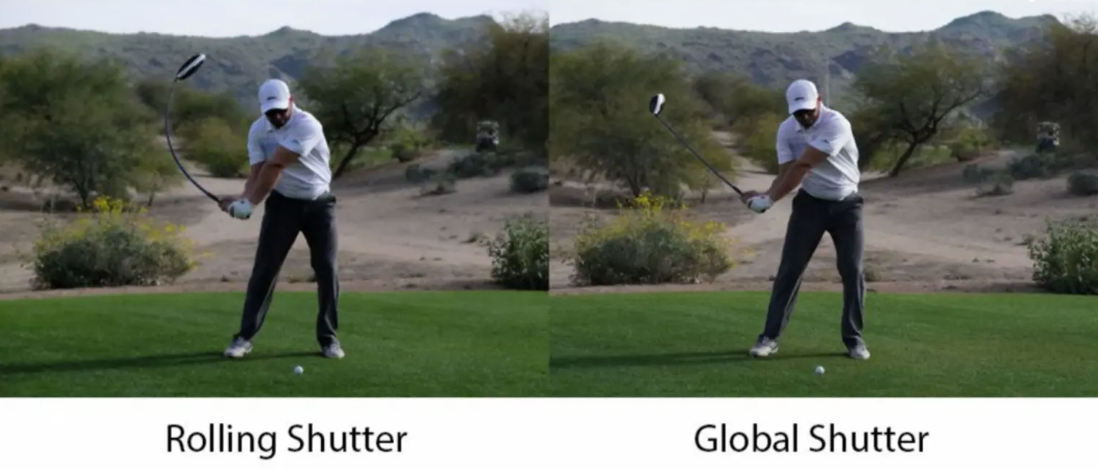
\includegraphics[width=0.82\textwidth]{images/rolling_shutter_revised.png}
\caption{原教材的快门对比示意：看球杆形状，不把照片当本次受控实拍}
\label{fig:v2-camera-shutter-photo}
\end{figure}
\begin{example}[把时序写成数值]
设图像速度为 800 pixel/s，单行曝光 2 ms，则曝光内位移约为 1.6 pixel；如果首末行曝光起点另外相差 6 ms，跨行对应的位置差约为 4.8 pixel。这两个量描述不同现象，缩短曝光不保证同时缩短读出时差。我们将在下面的 optics 中计算曝光位移，在“运动预算”练习中一起核对读出差。
\end{example}
\begin{conclusion}
传感器类型说明读出结构，快门类型说明曝光时序。光圈改变入光，曝光决定积分时间，增益放大已有信号。选运动相机先核对实际快门与读出条件；静态场景可以权衡分辨率和成本，不给所有卷帘产品套同一条结论。
\end{conclusion}

\subsubsection{准备一个可以反复检查的小实验}
本章完整项目在本卷 \path{examples/camera/calibration-lab-demo}。我们先用小数组算成像参数，再生成明确的模拟棋盘格，接着检测、标定、验证，最后接到 ROS 的保存和校正链路。模拟实验能排查单位与接口，却不能代替曝光、焦点和硬件同步的实拍验收。
\begin{example}[安装依赖并进入项目]
在 Ubuntu 22.04 / Humble 环境里使用系统 Python，避免把另一个虚拟环境的 cv2 混进 ROS。普通数值部分需要 NumPy、OpenCV 和 PyYAML；图形标定稍后再安装 ROS 包。
\begin{tbash}
sudo apt install python3-numpy python3-opencv python3-yaml
cd /你的教材目录/02-专项技术栈/examples/camera/calibration-lab-demo
python3 -c "import cv2,numpy,yaml; print(cv2.__version__,numpy.__version__)"
\end{tbash}
把路径换成实际位置，后面的短命令都从这个项目目录执行。记录命令输出的 OpenCV 和 NumPy 版本，后续实验使用同一个系统解释器。目录如下，输出放到 data/out，不覆盖教材源文件：
\begin{tbash}
calibration-lab-demo/
  optics.py            # 曝光、景深和单位计算
  format_gamma.py      # Bayer 与 Gamma 小数组
  noise.py             # 声明模型的加噪实验
  board.py             # 统一板规格与检测
  generate.py          # 已知几何模型的模拟图
  model_io.py          # 标定 YAML 保存与读取
  calibrate.py         # 多图标定与逐图误差
  validate.py          # 固定内参的独立图检查
  replay_ros.py        # 回放、参数服务和持久保存
  check_ros.py         # 原图/参数/校正输出核对
  stereo.py            # 双目几何与极线残差
  README.md
\end{tbash}
项目准备与命令实践由后面的噪声、格式和标定练习一起检查，不再出一题重复进入目录。
\end{example}

\subsubsection{噪声：别把“看着有颗粒”当成诊断}
图像噪点可能来自光子统计、读出电路、温度、坏点或传输/解码问题。高斯噪声（Gaussian noise）描述幅值分布；白噪声（white noise）描述相关性或频谱条件，两者不是同一个词换语言。读出噪声有时近似高斯，但不能凭图片外观确认全部来源。

泊松噪声（Poisson noise）可描述光子计数的散粒噪声。期望光子数为 $N$ 时，标准差约为 $\sqrt N$，相对标准差为 $1/\sqrt N$。从 100 增加到 400，绝对标准差从 10 变 20，相对噪声却从 10\% 降为 5\%。补光增加光子，增益放大已有值，它们不是等价操作。

乘性噪声可写成 $I'=I(1+\eta)$，扰动幅度随信号变化，这只是建模方式，不说明所有相机噪声都来自信道。椒盐噪声（salt-and-pepper noise）把一部分像素改到极低或极高；出现亮暗点还应查坏点和链路，不能先套滤波再宣布原因找到了。
\begin{figure}[H]
\centering
\begin{minipage}{0.30\textwidth}\centering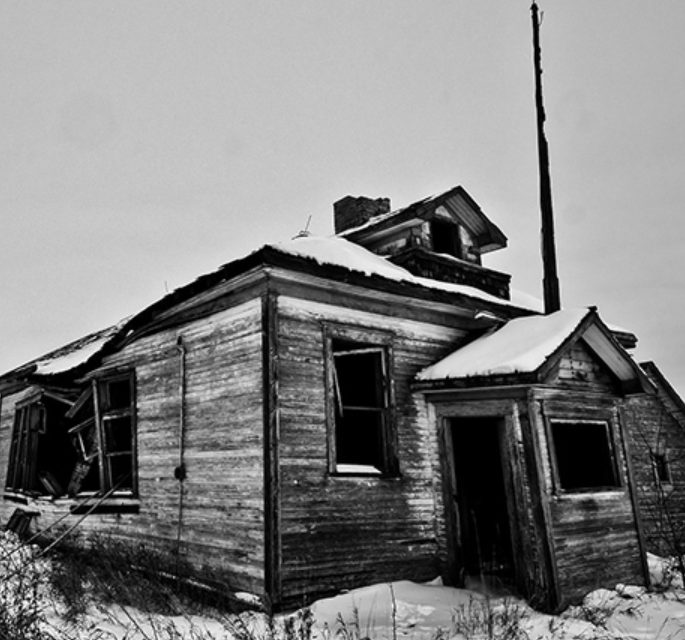
\includegraphics[width=\linewidth]{images/raw_revised.png}\\原图\end{minipage}\hfill
\begin{minipage}{0.30\textwidth}\centering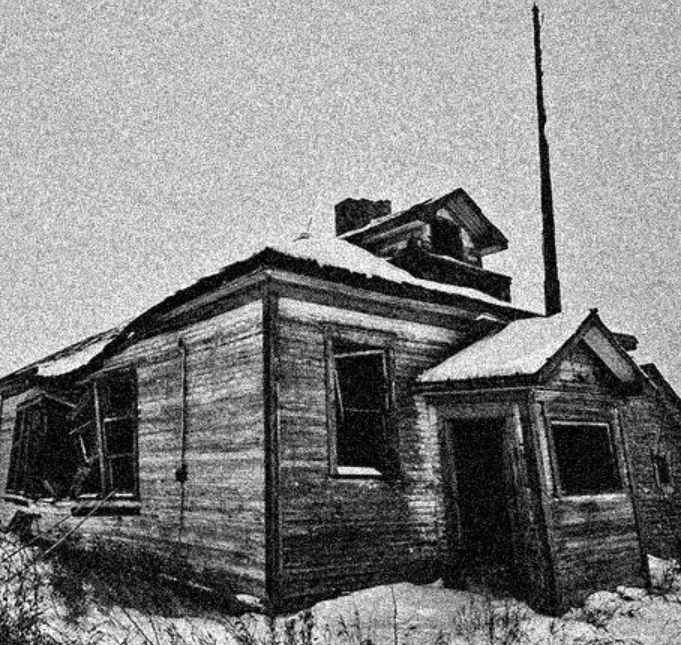
\includegraphics[width=\linewidth]{images/gaussian_revised.png}\\高斯示意\end{minipage}\hfill
\begin{minipage}{0.30\textwidth}\centering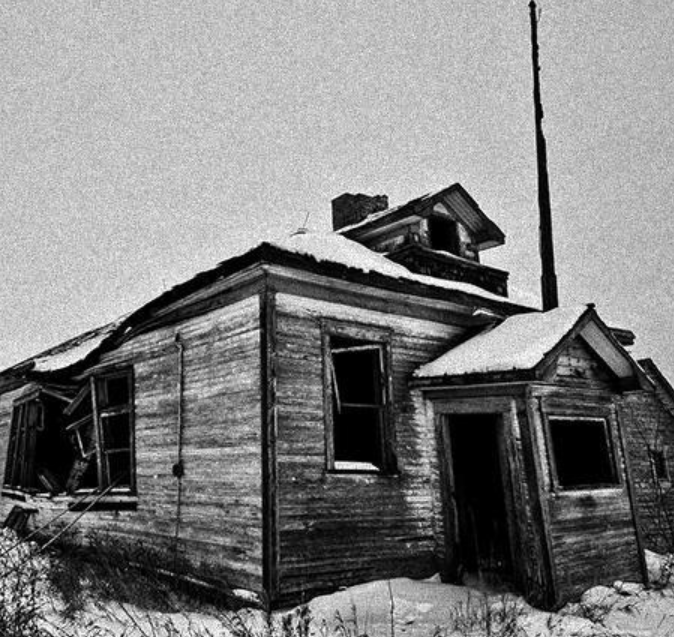
\includegraphics[width=\linewidth]{images/poisson_revised.png}\\泊松示意\end{minipage}

\smallskip
\begin{minipage}{0.30\textwidth}\centering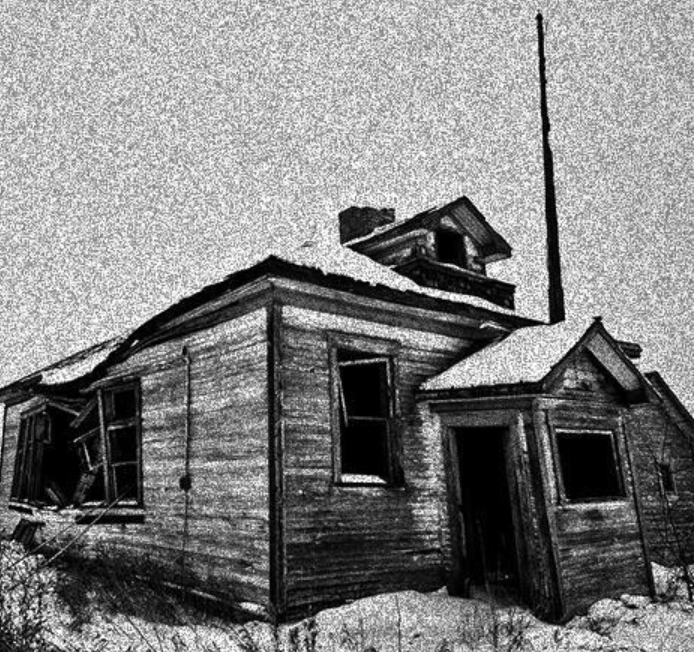
\includegraphics[width=\linewidth]{images/camera_multiplicative_revised.png}\\乘性示意\end{minipage}\hspace{0.06\textwidth}
\begin{minipage}{0.30\textwidth}\centering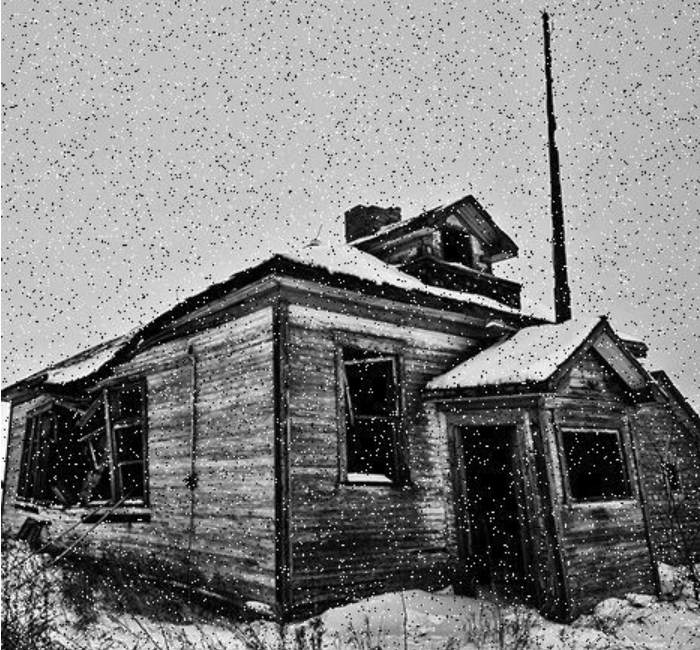
\includegraphics[width=\linewidth]{images/salt_revised.png}\\椒盐示意\end{minipage}
\caption{保留原教材五幅对照图；具体生成参数未知，不据它们倒推传感器噪声}
\label{fig:v2-camera-old-noise}
\end{figure}
\begin{example}[有参数的噪声实验]
noise 抽样 100000 次光子计数，再给同一灰度坡道加四种声明的噪声；随机种子固定，输出截到 0–255 并保存。坡道用于检查输入，不是相机实测。
\end{example}
\lstinputlisting[numbers=left,language=Python,basicstyle=\footnotesize\ttfamily,caption={noise.py}]{examples/camera/calibration-lab-demo/noise.py}
\begin{tbash}
python3 noise.py --photons 900 --output out/noise
\end{tbash}
通用形式是 \texttt{python3 noise.py [选项]}，photons 为期望光子数，output 为输出目录。本次理论标准差 30、相对值约 0.0333，抽样标准差约 30.015；不要求随机实验的小数等于理论值。滤波选择见 OpenCV 章，光照和读出问题仍需设备排查。
\begin{exercise}\label{ex:v2-camera-noise}
手算 N=900 的标准差和相对噪声，再运行 --photons 100 与 400。解释绝对噪声变大为何仍可能改善相对噪声，指出补光与增益的不同。
\end{exercise}

\subsubsection{像素格式与 Gamma：形状对了，颜色也要对}
彩色 Bayer 阵列每个位置只采一种颜色，典型 $2\times2$ 单元有两个 G、一个 R、一个 B；原始数据是单通道采样。不同起点形成 RGGB/BGGR 等排列，去马赛克（demosaicing）后才得到每像素三通道。Bayer 不是“.raw 后缀”的同义词，RAW 容器也可能有头部、位打包、黑电平和元数据。

RGB 每像素有红绿蓝三通道，OpenCV 常用 BGR 顺序。无填充的 640×480、8 位样本，Bayer8 为 307200 字节，RGB8 为 921600；10/12 位打包、行填充和 JPEG 压缩不能直接套这两个数。ROS 中还需核对 encoding、step 和 data 长度，前面的图像桥接章已有完整实验。

Gamma 是非线性亮度映射。本例约定 $y=x^{1/\gamma}$，$x=I/255$；gamma=2.2 提亮暗部，gamma=1 不变，小于 1 则压暗。另一些相机参数直接用指数，方向可能相反，先查文档。它不会恢复已经过曝或量化丢掉的细节，简单幂律也不等于完整 sRGB 编码。
\begin{example}[核对 Bayer 与查找表]
程序先造 8×6 RGGB：R=200、G=100、B=50，用 OpenCV 4.5 的 \texttt{COLOR\_BayerBG2BGR} 核对中心；这个两字母名称对应本例的 RGGB 排列，不能只看名字猜通道顺序。随后建立 256 项查找表（Look-Up Table，LUT），用 cv2.LUT 处理坡道。构表只做 256 次幂运算，不对每帧每像素重复求幂。
\end{example}
\lstinputlisting[numbers=left,language=Python,basicstyle=\footnotesize\ttfamily,caption={format\_gamma.py}]{examples/camera/calibration-lab-demo/format_gamma.py}
\begin{tbash}
python3 format_gamma.py --gamma 2.2 --output out/format
python3 format_gamma.py --gamma 1 --output out/identity
\end{tbash}
预期 Bayer 为 48 字节、BGR 为 144，中心 [50,100,200]；2.2 时 LUT[128]=186，1 时 identity=true。换阵列起点却不换代码，颜色就可能反了，形状正确也救不了。
\begin{figure}[H]
\centering
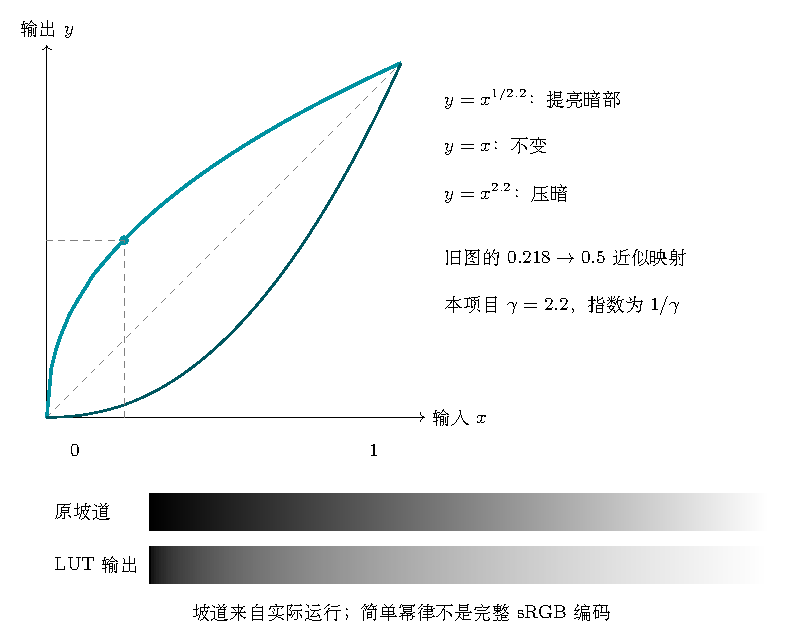
\includegraphics[width=0.94\textwidth]{images/camera_gamma_revised.pdf}
\caption{两种指数约定要分清；坡道使用本项目实际 LUT 输出}
\label{fig:v2-camera-gamma}
\end{figure}
\begin{exercise}\label{ex:v2-camera-format}
计算 1280×720 的 Bayer8/BGR8 字节，不计填充。解释 RGB/BGR 与 Bayer 排列是两种不同约定，说明文件大小为何可能不同。
\end{exercise}
\begin{exercise}\label{ex:v2-camera-gamma}
运行 gamma=1 核对完整坡道，再改为 0.5。说明暗部变化方向，以及为什么提亮饱和像素不能找回纹理。
\end{exercise}

\subsubsection{景深与焦段：不是“对过焦就一直清楚”}
对普通薄透镜近似，只有一个物平面严格合焦；离开它的点在像平面形成弥散圆（circle of confusion）。模糊在当前清晰度判据内，看起来仍够清楚，这段物方范围叫景深（depth of field）。像方允许的范围叫焦深（depth of focus），不要互换。容许弥散圆 $c$ 由成像、观察/检测要求等决定，不是所有系统都固定等于一个像元。
\begin{figure}[H]
\centering
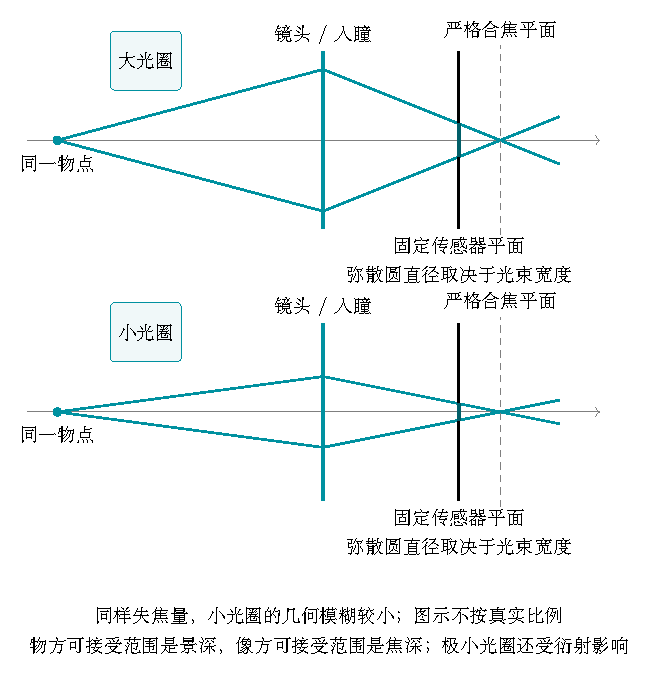
\includegraphics[width=0.94\textwidth]{images/camera_focus_revised.pdf}
\caption{合焦、可接受模糊与失焦；示意不按真实尺寸绘制}
\label{fig:v2-camera-focus}
\end{figure}
同样焦距、对焦距离和判据下，收小光圈通常增大几何景深，却也减少进光，极小光圈还受衍射影响。其他条件不变时，更长焦距通常让景深更浅，距离增大通常让景深更大；改变成像倍率或裁剪后，别只背结论就跳过条件。

\paragraph*{景深估算*}
沿用旧图的薄透镜关系，焦距 $f$、光圈数 $N$、弥散圆 $c$、物距 $s$ 采用相同长度单位，设 $h=f^2/(Nc)$，超焦距为 $H=h+f$。近、远界为
\[
s_{\mathrm{near}}=\frac{hs}{h+s-f},\qquad
s_{\mathrm{far}}=\frac{hs}{h-s+f}.
\]
远界分母不为正时取无穷，不输出负距离。前景深为 $s-s_{\mathrm{near}}$，后景深为 $s_{\mathrm{far}}-s$；有限远界下，后者通常较大。图 \ref{fig:v2-camera-dof} 保留旧图总景深与远距离近似；程序不模拟多片镜头和衍射。
\begin{figure}[H]
\centering
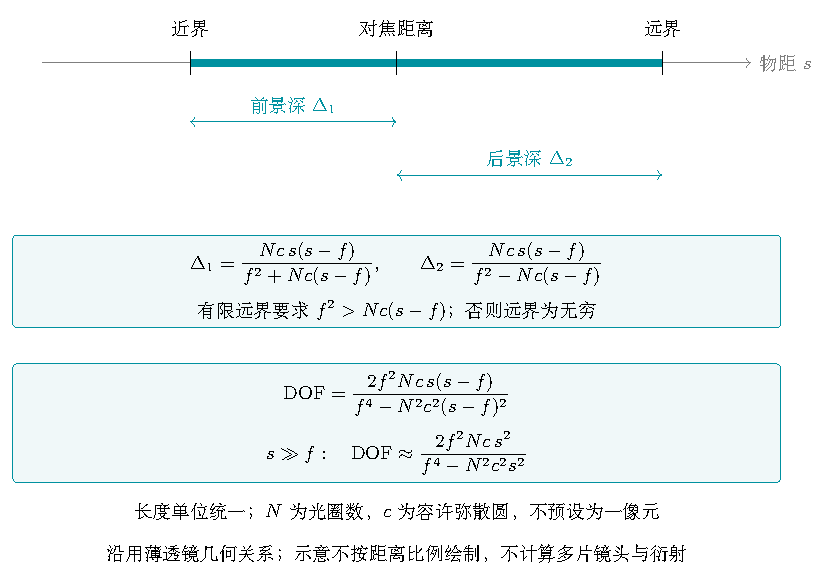
\includegraphics[width=0.94\textwidth]{images/camera_dof_revised.pdf}
\caption{前后景深、总景深与近似的条件}
\label{fig:v2-camera-dof}
\end{figure}
\begin{example}[把单位和边界写进程序]
optics 固定毫米、毫秒和 pixel/s，拒收非正/非有限参数；超过超焦距时 far=null 表示无穷。它还汇总后面运动、裁剪、双目和同步的手算值，覆盖小规模计算，不模拟硬件。
\end{example}
\lstinputlisting[numbers=left,language=Python,basicstyle=\footnotesize\ttfamily,caption={optics.py}]{examples/camera/calibration-lab-demo/optics.py}
\begin{tbash}
python3 optics.py
python3 optics.py --aperture 8
\end{tbash}
默认 $f=16$ mm、$N=4$、$c=0.01$ mm、$s=2000$ mm，H=6416 mm，近界约 1526.72、远界约 2898.55 mm；N=8 时 H=3216。实际清晰度仍需拍图确认。
\begin{exercise}\label{ex:v2-camera-dof}
运行 N=8 记录超焦距和近远界，再设 --distance 7000。解释 far=null，为什么不能说收小光圈在任何情况下都改善成像。
\end{exercise}

\subsubsection{运动预算与焦段选择}
现在把“不能太糊”变成一个数。图像速度近似恒定时，曝光位移 $b=vt$；最多容许 $b_{\max}$，则 $t\le b_{\max}/v$。$v$ 是 pixel/s，换成世界中的 m/s 还需要成像几何，不能直接混用。
\begin{example}[先算最长曝光，再在相机确认]
\begin{tbash}
python3 optics.py --speed 800 --exposure 2 --budget 1
python3 optics.py --speed 1200 --exposure 2 --budget 0.6
\end{tbash}
第一条位移 1.6 pixel、最长曝光 1.25 ms；第二条最长 0.5 ms。驱动范围、步长、触发与帧周期可能限制设置，填完还要读回并实拍。增益不改变同一曝光内的位移，只可能在亮度允许时帮助采用更短曝光。
\end{example}
\begin{exercise}\label{ex:v2-camera-motion}
手算 800 pixel/s、最多 1 pixel 的最长曝光，与输出核对。另算首末行差 6 ms 时的位置差，说明短曝光与短读出时间各自解决什么。
\end{exercise}

焦距决定视场与目标成像大小。同一传感器、距离和输出模式下，小角度近似中目标宽度与焦距成比例。换长焦能让目标更大，也让视野变窄；先想好最近距离能否看全，再检查接口、对焦、畸变和景深。卷三会接到实车选型，本章先做比例估算。
\begin{example}[从 8 mm 换到 12 mm]
原来宽 20 pixel 的同一目标，约变为 $20\times12/8=30$ pixel，optics 的 width\_8\_to\_12\_px 输出这一值。姿态、距离、像元和裁剪缩放不变才成立；近距离、离轴或畸变明显时重新投影。
\end{example}
\begin{exercise}\label{ex:v2-camera-lens}
估算上述宽度并列出不变条件。若只裁图再放大，为什么不能说相机收到的目标细节也增加了？
\end{exercise}
\begin{conclusion}
先用清晰度预算限制曝光，再用光圈、光照和增益权衡亮度。景深要说明距离与判据，焦段要兼顾像素与视场。格式与 Gamma 改变表达，不能修复曝光模糊、卷帘几何或丢掉的信息。
\end{conclusion}

\subsubsection{从棋盘格照片到内参与畸变}
镜头不是完美针孔，画面边缘直线可能弯曲；标定就是用一组几何参数说明空间点与像素关系。普通针孔用径向/切向畸变，鱼眼常用另一套模型。OpenCV 的 fisheye 四参数不是普通五参数的前四项，不能靠截数组转换。

我们优先用平整棋盘格：9×6 内角点对应 10×7 方格；25 mm 边长在米制程序中是 0.025。板固定在硬板上，实测横纵尺寸，固定工作分辨率、镜头与焦点，再采不同位置、距离和倾角。约 20–30 个有差异姿态可作实拍起点，覆盖不够再补；几百张相似正面图也不能代替倾斜约束。另留验证照片，别全部拿去拟合。
\begin{example}[生成可复现的模拟输入]
board 统一板规格与细化，generate 使用声明的 K/D/姿态渲染理想平面，再按畸变反向采样成原图。种子 2026，越出画面的板跳过，训练与验证按编号分开；front 为正面变体，left/right 为 0.12 m 基线的模拟双目。本次生成 83 张训练、15 张验证、12 张正面和 94 对双目图。truth.json 只记生成条件，标定不读取它。
\end{example}
\lstinputlisting[numbers=left,language=Python,basicstyle=\footnotesize\ttfamily,caption={board.py}]{examples/camera/calibration-lab-demo/board.py}
\lstinputlisting[numbers=left,language=Python,basicstyle=\footnotesize\ttfamily,firstline=1,lastline=37,caption={generate.py：模型与渲染}]{examples/camera/calibration-lab-demo/generate.py}
接着改变位置、距离和倾角，筛去越界图，按组保存；右相机的平移再减基线。所有分组仍是模拟输入，没有加入曝光噪声或传感器读出。
\lstinputlisting[numbers=left,language=Python,basicstyle=\footnotesize\ttfamily,firstline=38,firstnumber=38,caption={generate.py：采样与分组}]{examples/camera/calibration-lab-demo/generate.py}
\begin{tbash}
python3 generate.py --output data
python3 calibrate.py --images data/train --output out
python3 calibrate.py --images data/front --output out/front
\end{tbash}
输出目录的同名图会写入，首次练习用新目录。--images 为输入 PNG 目录，--square 为米制边长，--output 为结果目录。calibrate 检查模式、跳过未检出的板，至少十张有效图才求解；十张只是演示下限，不是合格标准。

这里固定 k3=0，保留 k1/k2/p1/p2，稍后 ROS 命令也明确用两个径向系数，避免不同模型只比 RMS。逐图残差与总 RMS 存 metrics，K/D、尺寸、方格与平移存 NPZ，另写标定 YAML。
\lstinputlisting[numbers=left,language=Python,basicstyle=\footnotesize\ttfamily,caption={calibrate.py}]{examples/camera/calibration-lab-demo/calibrate.py}
本次多姿态 83 张 RMS 约 0.255 pixel，$f_x\approx559.70$；正面 12 张也只有约 0.263 pixel，但 $f_x\approx2493.39$，远离生成的 560。低残差只说明能拟合这些图，不代表内参可信，约束不足不能靠“拍得更多”自动解决。
\begin{exercise}\label{ex:v2-camera-calibrate}
运行 train/front，比较有效数、RMS、K/D 与生成条件，再用各自参数验证 validation/000.png。说明为何不能只按训练 RMS 排名；实拍时保留独立验证和模式记录。
\end{exercise}
\subsubsection{读懂标定结果：模型、采集与误差}
\label{sec:camera-calibration-detail}

相机标定（camera calibration）建立三维点与像素坐标之间的关系。先分清三类量：内参描述相机怎样成像；畸变系数描述镜头偏离理想模型的程度；外参描述两个坐标系的相对位姿。单目标定输出的每张棋盘格位姿，是该次拍摄中“标定板到相机”的变换，不能直接当成“相机到机器人底盘”的固定安装外参。后者需要另做外参或手眼标定。

\paragraph*{从空间点到像素}
令相机坐标系中的点为 $(X_c,Y_c,Z_c)$，且 $Z_c>0$。归一化坐标为 $x=X_c/Z_c$、$y=Y_c/Z_c$。忽略像素轴倾斜时，内参矩阵为
\[
K=\begin{bmatrix}f_x&0&c_x\\0&f_y&c_y\\0&0&1\end{bmatrix},
\qquad u=f_xx+c_x,\quad v=f_yy+c_y.
\]
$f_x,f_y$ 的单位是像素，不是镜头标称的毫米；$c_x,c_y$ 是主点位置，通常接近图像中心，但不应强行当成中心。ROS 光学坐标系通常约定 $x$ 向右、$y$ 向下、$z$ 向前，不能与机器人机体坐标轴混用。

普通针孔模型常使用五个畸变系数 $D=(k_1,k_2,p_1,p_2,k_3)$。令 $r^2=x^2+y^2$，则
\begin{align*}
L&=1+k_1r^2+k_2r^4+k_3r^6,\\
x_d&=xL+2p_1xy+p_2(r^2+2x^2),\\
y_d&=yL+p_1(r^2+2y^2)+2p_2xy.
\end{align*}
再将 $x_d,y_d$ 代入像素公式。三个 $k$ 描述径向变化，两个 $p$ 描述切向变化。其他模型可能使用更多参数；鱼眼模型的四个系数不是上述五参数模型的前四项，不能靠截取数组转换。

\begin{example}[裁剪、缩放后怎样改内参]
假设原图为 $1280\times960$，$f_x=f_y=800$、$(c_x,c_y)=(640,480)$。从左上角 $(100,50)$ 裁取区域，再把裁出的图像按坐标比例缩小到一半。在使用 $u'=s_x(u-u_0)$、$v'=s_y(v-v_0)$ 的坐标约定下：
\begin{tpython}
fx, fy, cx, cy = 800., 800., 640., 480.
u0, v0, sx, sy = 100., 50., 0.5, 0.5
new_K = [[sx*fx, 0., sx*(cx-u0)],
         [0., sy*fy, sy*(cy-v0)], [0., 0., 1.]]
assert new_K == [[400., 0., 270.], [0., 400., 215.], [0., 0., 1.]]
print(new_K)
\end{tpython}
纯图像坐标变换不改变原镜头的归一化畸变模型；但要同步更新尺寸、ROI 和相应投影矩阵。具体缩放实现若采用半像素中心约定，还要按该实现修正主点。切换传感器模式、对焦、变焦或更换镜头并非简单缩放，应重新确认或重新标定。
\end{example}

\paragraph*{怎样采到有效的数据}
平面棋盘格的张正友标定法先利用多视角平面映射约束内参，再联合优化畸变和每张图的位姿。多拍几百张几乎相同的正面图，不等于获得了足够的几何约束。
\begin{enumerate}
\item 将标定板牢固贴在平整硬板上，实测横纵方格边长，检查打印是否被拉伸。9×6 个内角点对应 10×7 个方格；25 mm 在以米为单位的程序中写 0.025。
\item 固定实际工作分辨率、镜头、焦距和对焦位置。关闭会改变几何成像的自动对焦，曝光以角点清晰、黑白区域不过曝为准。
\item 让完整棋盘格出现在中心、四角和边缘，改变距离与俯仰、偏航角；近景覆盖较大面积，远景保留足够清晰的方格。倾斜要有差异，但不能倾斜到角点难以定位。
\item 每个姿态停稳后采集，尤其避免卷帘快门下晃动标定板。先采集约 20--30 个有差异的姿态作为教学起点，再按覆盖和误差补采；张数不是合格证。
\item 另外保留数张清晰、不同位置与倾角的照片作验证，不让它们参与参数拟合。记录相机编号、镜头、分辨率、标定板尺寸和采集日期。
\end{enumerate}

\paragraph*{重投影误差怎样算、怎样看}
把标定板角点用估计的位姿、内参和畸变重新投影到图像，与检测到的角点相减，得到残差。对于总计 $N$ 个二维角点，本章使用
\[
\mathrm{RMS}=\sqrt{\frac{1}{N}\sum_{i=1}^{N}\left\|\hat{\boldsymbol p}_i-\boldsymbol p_i\right\|_2^2}.
\]
单位是像素。不要将所有二维坐标分量的平均误差与这个定义混用，也不要只比较不同分辨率下的数值大小。应同时查看逐图误差、边缘残差、参数合理性、重复标定的稳定性和未参与拟合的图像。某张照片误差很大时先检查模糊、错检或板面弯曲；不能为了降低平均数盲目删除全部边缘照片。

\begin{example}[检查独立照片并生成去畸变图]
先运行前节程序生成 calibration.npz，再保存一张未参与标定的同分辨率照片为 validation.png。以下程序估计该照片中标定板的位姿，保持原 $K,D$ 不变，计算残差并输出 undistorted.png：
\begin{tpython}
import cv2
import numpy as np

data = np.load("calibration.npz")
K, D = data["K"], data["dist"]
img = cv2.imread("validation.png")
if img is None:
    raise ValueError("找不到 validation.png")
size = (img.shape[1], img.shape[0])
if tuple(data["size"]) != size:
    raise ValueError("验证图与标定图分辨率不一致")
gray = cv2.cvtColor(img, cv2.COLOR_BGR2GRAY)
ok, corners = cv2.findChessboardCorners(gray, (9, 6))
if not ok:
    raise ValueError("未找到完整的 9x6 内角点")
criteria = (cv2.TERM_CRITERIA_EPS + cv2.TERM_CRITERIA_MAX_ITER, 30, 0.001)
corners = cv2.cornerSubPix(gray, corners, (11, 11), (-1, -1), criteria)
obj = np.zeros((54, 3), np.float32)
obj[:, :2] = np.mgrid[0:9, 0:6].T.reshape(-1, 2) * 0.025
ok, rvec, tvec = cv2.solvePnP(obj, corners, K, D)
if not ok:
    raise ValueError("位姿求解失败")
pred, _ = cv2.projectPoints(obj, rvec, tvec, K, D)
err = np.linalg.norm(pred.reshape(-1, 2) - corners.reshape(-1, 2), axis=1)
print("验证 RMS / pixel:", np.sqrt(np.mean(err**2)))
print("最大角点残差 / pixel:", err.max())
new_K, roi = cv2.getOptimalNewCameraMatrix(K, D, size, 1.0, size)
out = cv2.undistort(img, K, D, None, new_K)
if not cv2.imwrite("undistorted.png", out):
    raise IOError("无法保存图像")
np.savez("rectified_model.npz", K=new_K, size=size, roi=roi)
\end{tpython}
验证图的位姿仍由该图估计，所以这是固定内参后的泛化检查，并非独立真值精度。检查校正图中直线是否变直、边缘是否过度拉伸；保留全视场时出现黑边可能是正常现象。程序没有裁掉 ROI。后续在该校正图上做 PnP，应使用 new\_K 和零畸变；在原图上做 PnP，则使用原 $K,D$，不要重复去畸变。
\end{example}

\begin{exercise}
原图的 $f_x=1000,c_x=640$，先从左侧裁去 80 pixel，再按本节坐标约定缩小到一半，新的 $f_x,c_x$ 是多少？为什么不能只修改图像宽高？
\end{exercise}

\subsubsection{ROS2 的 camera\_calibration 标定流程}
\label{sec:ros2-camera-calibration}

本节使用 Ubuntu 22.04 / ROS2 Humble。\texttt{camera\_calibration} 属于 image\_pipeline，负责从图像求参数；\texttt{camera\_info\_manager} 是供驱动使用的参数管理库；\texttt{image\_proc} 根据图像和参数生成校正图。安装管理库不会让任意驱动自动具备参数加载服务。

\begin{center}
\begin{tabular}{p{0.31\textwidth}p{0.60\textwidth}}
\toprule[1.5pt]
消息或字段 & 作用 \\
\midrule[1pt]
\nolinkurl{sensor_msgs/msg/Image} & 原始图像及其时间戳、光学坐标系名称。\\
\nolinkurl{sensor_msgs/msg/CameraInfo} & 与该图像模式对应的几何参数。\\
\texttt{k / d} & 原始图像的 $3\times3$ 内参及畸变数组；同时检查 distortion\_model。\\
\texttt{r / p} & 校正旋转与 $3\times4$ 投影矩阵；R 不是机器人安装外参。\\
\texttt{width / height} & 参数对应的标定图像尺寸；ROI、binning 也需一致。\\
\nolinkurl{set_camera_info} & 驱动提供的写入服务，类型为 SetCameraInfo。\\
\bottomrule[1.5pt]
\end{tabular}
\end{center}
消息字段使用小写 k、d、r、p，文档常记作 $K,D,R,P$。未标定时 $K_{00}=0$ 是约定的识别信号；不能把全零参数交给校正程序。原始和校正图要使用各自对应的几何模型。

\begin{example}[安装、核对话题并启动单目标定]
先按相机厂商或驱动文档启动真实相机，使其发布未去畸变的 \texttt{/camera/image\_raw}。驱动与设备相关，本节不假定某一厂商的启动命令。需要能显示 OpenCV 窗口的图形会话；无桌面的 SSH 会话不能直接显示此界面。
\begin{tbash}
sudo apt update
sudo apt install ros-humble-camera-calibration ros-humble-image-proc \
  ros-humble-camera-info-manager ros-humble-rqt-image-view
source /opt/ros/humble/setup.bash
ros2 run camera_calibration cameracalibrator --help
ros2 topic info /camera/image_raw --verbose
ros2 topic hz /camera/image_raw
ros2 service list -t
\end{tbash}
结束频率观测后继续。确认输入类型是 Image 而非 CompressedImage，并记录实际的设置服务名。通用形式为 \texttt{ros2 run camera\_calibration cameracalibrator [标定选项] --ros-args [重映射]}。
\begin{center}
\begin{tabular}{p{0.34\textwidth}p{0.57\textwidth}}
\toprule[1.5pt]
参数 & 作用 \\
\midrule[1pt]
\texttt{--size 9x6} & 棋盘格内角点的列数和行数。\\
\texttt{--square 0.025} & 单个方格边长，单位米。\\
\texttt{--camera\_name front} & 保存到标定文件中的相机名，应与驱动配置匹配。\\
\texttt{--no-service-check} & 跳过启动时的写入服务检查，不会创建服务。\\
\texttt{--approximate 0.01} & 双目配对允许的时间差，单位秒。\\
\bottomrule[1.5pt]
\end{tabular}
\end{center}
其余选项查看本机 --help。Humble 标定器默认只优化两个径向系数；与前节 OpenCV 默认配置比较时，要先统一模型和固定参数选项，不能只比较 RMS。对 9×6 内角点、25 mm 方格的棋盘格执行：
\begin{tbash}
ros2 run camera_calibration cameracalibrator \
  --size 9x6 --square 0.025 --camera_name front \
  --ros-args -r image:=/camera/image_raw \
  -r camera/set_camera_info:=/camera/set_camera_info
\end{tbash}
若驱动没有写入服务，在 --ros-args 之前添加 \texttt{--no-service-check}，先走保存文件的路径；不要点击 COMMIT 并期待驱动自动支持它。
\end{example}

\paragraph*{采集、求解、保存和部署}
\begin{enumerate}
\item 按前节采集方法移动标定板。界面的 X、Y、Size、Skew 表示位置、尺寸与倾斜覆盖；停稳后确认角点被识别，不要一直快速晃动。
\item CALIBRATE 可用后开始求解，等待完成，再检查校正预览和输出参数。界面允许点击只表示满足采样条件，仍需质量验证。
\item SAVE 将结果和采样图像保存到归档文件；Humble 实现默认写入 \nolinkurl{/tmp/calibrationdata.tar.gz}。每次保存后及时复制，避免下次实验覆盖或临时目录清理。
\item COMMIT 尝试调用驱动的 SetCameraInfo 服务。检查返回的 success 和 status\_message 以及驱动日志；调用成功后仍需重启驱动验证是否真正持久保存。
\item 无写入服务时，从归档中取得 YAML，再使用驱动支持的标定文件配置加载。常见参数名是 camera\_info\_url，但名称、相机名要求和是否支持运行时更新以实际驱动为准。
\end{enumerate}

\begin{example}[保存归档并验证重新加载]
点击 SAVE 后在终端执行，独立目录由 mktemp 创建：
\begin{tbash}
mkdir -p "$HOME/calibrations"
calib_dir=$(mktemp -d "$HOME/calibrations/front.XXXXXX")
cp /tmp/calibrationdata.tar.gz "$calib_dir/"
tar -tzf "$calib_dir/calibrationdata.tar.gz"
tar -xzf "$calib_dir/calibrationdata.tar.gz" -C "$calib_dir"
find "$calib_dir" -name '*.yaml'
echo "$calib_dir"
\end{tbash}
以归档实际内容为准选取单目 YAML（常见为 ost.yaml），不要误拿双目的另一侧文件。文件通常包含 image\_width、image\_height、camera\_name、camera\_matrix、distortion\_model、distortion\_coefficients、rectification\_matrix 和 projection\_matrix；它不是 ROS 节点的 ros\_\_parameters 配置，不能直接假定可用 --params-file 载入。

对提供 camera\_info\_url 参数的驱动，把该参数设为实际文件的绝对 URL，例如 \nolinkurl{file:///home/student/calibrations/front.yaml}；这是格式示例，必须换成上面生成的真实路径。重启驱动后执行：
\begin{tbash}
ros2 topic echo /camera/camera_info --once
ros2 launch image_proc image_proc.launch.py namespace:=camera
\end{tbash}
确认 CameraInfo 尺寸与输入模式匹配，k 中焦距非零，d 和模型与保存文件一致。另一个加载环境的终端运行：
\begin{tbash}
ros2 run rqt_image_view rqt_image_view
\end{tbash}
选择 \texttt{/camera/image\_rect}；彩色链路可查看 \texttt{/camera/image\_rect\_color}。比较原图和校正图中的直线及边缘，记录时间戳与 frame\_id。驱动必须以匹配时间戳发布图像和 CameraInfo；仅在终端看见过一次参数，不代表校正节点能同步到它。
\end{example}

\begin{note}
黑屏或无角点时按顺序检查：原图是否在发布、重映射是否正确、域和 QoS 是否兼容、图形会话是否可用、内角点数是否正确、图像是否清晰。没有校正图时再检查 CameraInfo、时间戳和参数尺寸。先启动驱动再启动标定工具；不同 Humble 补丁版本的 QoS 处理可能不同，使用 topic info --verbose 查看实际端点，不能只看话题名。
\end{note}
\begin{exercise}
驱动只有原图话题，没有 SetCameraInfo 服务。写出完成标定并保存结果的步骤；为什么加入 --no-service-check 后，仍不能保证重启驱动就有正确的 CameraInfo？
\end{exercise}

\subsubsection{双目标定与交付检查}
双目标定不仅求两侧内参，还要求相机之间的固定旋转和平移。两台相机必须固定相对位置，并同时看到同一块标定板。分别完成两次单目标定，不能得到它们之间的基线。相机、镜头或安装支架移动后要重新检查外参。

\begin{example}[启动双目交互标定]
先让两侧驱动发布同分辨率原始图像及各自的参数服务，再运行：
\begin{tbash}
ros2 run camera_calibration cameracalibrator \
  --size 9x6 --square 0.025 \
  --ros-args -r left:=/left/image_raw -r right:=/right/image_raw \
  -r left_camera/set_camera_info:=/left/set_camera_info \
  -r right_camera/set_camera_info:=/right/set_camera_info
\end{tbash}
默认按相同时间戳配对。无硬件同步的静态教学实验，可在 --ros-args 之前增加 \texttt{--approximate 0.01}，允许最多约 10 ms 的时间配对容差；它不会校正曝光时差，也不能代替硬件同步。采集时保持板面与相机静止再取样，且两侧都要有清晰角点。保存两侧结果，检查校正后对应角点的纵坐标是否接近，并检查基线与实测安装距离是否相符。
\end{example}

标准水平双目约定下，右侧投影矩阵包含 $P_{03}=-f_xB$，可据此核对基线 $B=-P_{03}/P_{00}$，单位由标定板尺寸决定。该关系针对校正后的标准水平双目模型；不是任意矩阵中都能直接抽出相机间距离。相机到云台、底盘或 IMU 的外参仍需另外标定并通过 TF 管理。

\begin{conclusion}
\begin{itemize}
\item 标定资料要同时交付原始样本、板参数、相机模式、结果文件、误差记录和独立验证图。
\item SAVE 保存文件，COMMIT 请求驱动写入，驱动重启后正确发布 CameraInfo 才能证明部署链路成立。
\item 原图使用原 $K,D$，校正图使用校正后的投影模型；ROI 与缩放也要计入。
\item 单目位姿、双目相对外参、机器人安装外参是不同任务；时间同步误差不能靠内参标定消除。
\end{itemize}
\end{conclusion}
\begin{exercise}
标准水平双目的右侧 $P_{00}=800$ pixel、$P_{03}=-96$ pixel\,m，基线是多少？若两帧曝光相差 10 ms，--approximate 能否消除运动目标的几何偏差？
\end{exercise}

\begin{note}
接口及命令按 ROS2 Humble 的官方源码核对：
\url{https://github.com/ros-perception/image_pipeline/tree/humble/camera_calibration}；
\url{https://github.com/ros-perception/image_pipeline/blob/humble/image_proc/launch/image_proc.launch.py}。
CameraInfo 的字段定义见
\url{https://docs.ros.org/en/humble/p/sensor_msgs/msg/CameraInfo.html}。
OpenCV 针孔模型与标定接口见
\url{https://docs.opencv.org/4.x/d9/d0c/group__calib3d.html}。
\end{note}


\subsubsection{HDR 与同步：选读也要分清代价*}
高动态范围（High Dynamic Range，HDR）可利用多曝光融合或传感器模式覆盖更大亮度范围。不过多帧不同时拍，运动物体融合后可能重影，等待和处理也增加延迟。它帮助避免部分饱和，不保证每个算法都受益；专用模式按实际文档确认。

多相机或相机/IMU 要有可比较的时间基准。硬件触发、设备时钟同步、主机接收时间和软件配对解决不同问题：同一触发也要核对实际曝光延迟，接收时间可能含传输/排队误差，按时间戳选最近帧不会让曝光同时发生。
\begin{example}[算清差几毫秒意味着什么]
optics 中 sync\_error\_m 用 3 m/s 与 8 ms 得 0.024 m，hdr\_shift\_px 用 1000 pixel/s 与 10 ms 得 10 pixel。下面的完整计算先统一秒与毫秒：
\begin{tpython}
speed_m_s, dt_s = 3.0, 1.008-1.000
assert abs(speed_m_s*dt_s-.024) < 1e-12
speed_px_s, dt_ms = 1000., 10.
assert speed_px_s*dt_ms/1000 == 10.
print(speed_m_s*dt_s, speed_px_s*dt_ms/1000)
\end{tpython}
这不是 HDR 实机测试；真机保存曝光与时间戳，在运动场景确认融合和时延。
\end{example}
\begin{exercise}\label{ex:v2-camera-hdr}
算出上述 HDR 错位，解释重影与过曝的不同；列出实际同步验证要记录的时钟来源、曝光时刻和接收时刻。
\end{exercise}
